
\documentclass[10pt,article]{memoir}

\usepackage[utf8]{inputenc}
\usepackage{hyperref}
\usepackage{microtype}
\usepackage{letltxmacro}
\usepackage[lining]{ebgaramond}
\usepackage[cmintegrals,cmbraces]{newtxmath}
\usepackage{ebgaramond-maths}
\usepackage{booktabs}
\usepackage{mathtools}
\usepackage{amssymb}
\usepackage{tikz}
\usepackage{enumitem}
\usepackage{rotating}
\renewcommand{\thefootnote}{\color{red}\arabic{footnote}}
\usepackage{placeins}
\usepackage[textsize=small, linecolor=magenta, bordercolor=magenta,
            backgroundcolor=magenta, textwidth=3cm]{todonotes}

\urlstyle{sf}
\makeatletter
    \let\UrlSpecialsOld\UrlSpecials
    \def\UrlSpecials{\UrlSpecialsOld\do\/{\Url@slash}\do\_{\Url@underscore}}%
    \def\Url@slash{\@ifnextchar/{\kern-.11em\mathchar47\kern-.2em}%
        {\kern-.0em\mathchar47\kern-.08em\penalty\UrlBigBreakPenalty}}
        \def\Url@underscore{\nfss@text{\leavevmode \kern.06em\vbox{\hrule\@width.3em}}}
\makeatother
\captionnamefont{\small\bfseries}
\captiontitlefont{\small}
\newsubfloat{figure}

\newenvironment{wideMinipage}
{ \vskip 1\baselineskip
  \noindent   
  \checkoddpage% 
  \ifoddpage%
     \hspace*{-3em}%
  \else%
     \hspace*{-3em}%
  \fi%
  \begin{minipage}{1\textwidth + 6em}
}
{ 
    \end{minipage}
    \vskip 1\baselineskip
}

\makeatletter
    \renewcommand{\@todonotes@drawMarginNoteWithLine}{%
    \begin{tikzpicture}[remember picture, overlay, baseline=-0.75ex]%
        \node [coordinate] (inText) {};%
    \end{tikzpicture}%
    \marginpar[{% Draw note in left margin
        \@todonotes@drawMarginNote{r}%
        \@todonotes@drawLineToLeftMargin%
    }]{% Draw note in right margin
        \@todonotes@drawMarginNote{l}%
        \@todonotes@drawLineToRightMargin%
    }%
    }
    \renewcommand{\@todonotes@drawMarginNote}[1]{
        \makebox[\marginparwidth][#1]{\begin{tikzpicture}[remember picture,baseline=(X.base)]%
            \node(X){\vphantom{X}};%
            \draw node[notestyle,font=\@todonotes@sizecommand,anchor=north] (inNote) at (X.north)%
                {\@todonotes@text};%
            \if@todonotes@authorgiven%
                \draw node[notestyle,font=\@todonotes@sizecommand,anchor=north] (inNote) at (X.north)%
                    {\@todonotes@sizecommand\@todonotes@author};%
                \node(Y)[below=of X]{};%
                \draw node[notestyle,font=\@todonotes@sizecommand,anchor=north] (inNote) at (X.south)%
                    {\@todonotes@text};%
            \else%
                \draw node[notestyle,font=\@todonotes@sizecommand,anchor=north] (inNote) at (X.north)%
                    {\@todonotes@text};%
            \fi%
        \end{tikzpicture}%
    }}
\makeatother
\LetLtxMacro{\oldtodo}{\todo}
\renewcommand{\todo}[1]{{\color{magenta}\oldtodo[fancyline]{\color{white}\textsf{#1}}}}
\newcommand{\inlinetodo}[1]{{\color{magenta}\oldtodo[inline]{\color{white}\textsf{#1}}}}

\setsecheadstyle{\LARGE}
\setsubsecheadstyle{\large}
\setsubsubsecheadstyle{\itshape}
\setparaheadstyle{\normalsize\scshape\liningnums}
\counterwithout{figure}{chapter}
\counterwithout{table}{chapter}
\captionnamefont{\textsf\small}
\captiontitlefont{\textsf\small}
\let\thempfootnote\thefootnote


\begin{document}

\begin{center}
{\LARGE\noindent Predicting off-target binding with confidence using Conformal
Prediction}
\end{center}

\begin{center}
\noindent
\begin{tabular}{ccc}
Samuel Lampa\,$^{1,*}$  & Jonathan Alvarsson\,$^{1}$ &  Staffan Arvidsson\,$^{1}$ \\
 Arvid Berg\,$^{1}$ &Ernst Ahlberg\, & Ola Spjuth\,$^{1}$ \\
\end{tabular}
\end{center}

\noindent
\begin{minipage}{1.1\textwidth}
\noindent\footnotesize $^1$Pharmaceutical Bioinformatics group, Department of Pharmaceutical Biosciences, Uppsala University, Uppsala, Sweden \\ 
\noindent\footnotesize $^2$Predictive Compound ADME \& Safety, Drug Safety \& Metabolism, AstraZeneca IMED Biotech Unit, Mölndal, Sweden \\ 
\end{minipage}


\def\keyFont{\fontsize{8}{11}\helveticabold }
\def\firstAuthorLast{Lampa {et~al.}} %use et al only if is more than 1 author
\def\Authors{Samuel Lampa\,$^{1,*}$, Jonathan Alvarsson\,$^{1}$, Staffan Arvidsson\,$^{1}$, Arvid Berg\,$^{1}$, Ernst Ahlberg\,$^{2}$  and Ola Spjuth\,$^{1}$}
\def\Address{$^{1}$Pharmaceutical Bioinformatics group, Department of Pharmaceutical Biosciences, Uppsala University, Uppsala, Sweden\\
$^{2}$Predictive Compound ADME \& Safety, Drug Safety \& Metabolism, AstraZeneca IMED Biotech Unit, M"olndal, Sweden}
\def\corrAuthor{Corresponding Author}

\def\corrEmail{samuel.lampa@farmbio.uu.se}

\begin{abstract}
\noindent
Panels of ligand-based models are widely used in drug discovery to obtain an
early indication of potential off-target predictions that could be linked
to drug efficacy and safety. Another application is to combine models into
a profile allowing to compare and search for compounds with similar
profile. Most contemporary methods and implementations however lack valid
measures of confidence in predictions, yielding only point predictions. We
here describe the use of conformal prediction for predicting off-target
interactions based on data from the ExCAPE database about 31 binding
targets, selected for their value in broad early hazard assessment. We used
support vector machines, with chemical described by the signature molecular
descriptor, to train predictive models.  Prediction results from the
resulting models are presented as prediction intervals, as customary in
conformal prediction. The full pre-processing and model training process is
openly available as a scientific workflow on github, rendering it fully
reproducible. The resulting models are published online and are available
via a graphical web interface and an OpenAPI interface for programmatic
access.

%\tiny
 %\keyFont{ \section{Keywords:} drug discovery, predictive modelling, conformal prediction, machine learning, off-target, adverse effects} %All article types: you may provide up to 8 keywords; at least 5 are mandatory.
\end{abstract}

\section*{Introduction}

%Introduce off target binding as a problem, and the value of predictions

Off-target pharmacology and polypharmacology has big implications on drug
efficacy and safety, and prediction of target binding profiles for ligands is
an important task that can aid early drug discovery~\cite{Bowes2012}. Drugs
often does not interact with just one target but with multiple
targets~\cite{hopkins2008network}. However, available methods for ligand-based
target profiling often do not offer valid measures of confidence in
predictions. We present an approach for ligand-based target profiling using a
confidence framework, delivering target profiles with confidence score for the
predictions of whether a query compound interact with each target. The
confidence scores are calculated using the Conformal Prediction
methodology~\cite{Vovk2005}, with support vector machines for modeling and
chemical structures described by the molecular signature
descriptor~\cite{Faulon2003}. The molecular signatures have previously been
sucessfully used for ligand-based target prediction~\cite{alvarsson2014ligand}
We study profiles for different sets of targets, including a subset of the
minimal panel of 44 targets for broad early hazard assessment suggested
by~\cite{Bowes2012}, but also the applicability of larger as well as focused
target sets.

\todo{Expand the intro above which is just taken from the abstract}

%Prior art - what has been done before?
Earlier studies...

%What is the motivation for the study, and what will we describe in this manuscript
In this manuscript we...

%%%%%%%%%%%%%%%%%%
%Methods
%%%%%%%%%%%%%%%%%%
\section*{Methods}

\subsection{Training data}

A scientific workflow was constructed to automate the entire data preprocessing.
The first step comprised extracting data on binding association between ligands and targets from the database ExcapeDB~\cite{Sun2017}, more specifically the columns Gene name, Original entry ID (PubChem CID or CHEMBL ID), SMILES and Activity flag. This was performed early in the workflow to make subsequent data transformation steps more performant, given the relative large size of the
uncompressed ExcapeDB data file (18 GB).
%
From the extracted dataset, all rows for which there existed rows with a conflicting
activity value, were completely removed.
% (See \href{https://github.com/pharmbio/ptp-project/blob/c529cf/exp/20180426-wo-drugbank/wo_drugbank_wf.go#L239-L246}{here}).

A subset of the panel of 44 binding targets as suggested in \cite{Bowes2012}
was selected for inclusion in the study. The selection was based on that targets
should have at least 100 associated and at least 100 non-associated compounds. 
In addition some targets were excluded for which data was not found in ExcapeDB, this is described in detail below.
%
Some of the gene ids used in \cite{Bowes2012} were not found in their exact
form in the ExcapeDB dataset. To resolve this, PubMed was consulted to find
synonymous gene IDs with the following replacements done:
%
\textit{KCNE1} was replaced with \textit{MINK1} which is present in ExcapeDB.
\textit{CHRNA1} (coding for the $\alpha1$ subunit of the Acetylcholine
receptor) is excluded, as it is not present in the dataset (\textit{CHRNA4},
coding for the $\alpha4$ subunit of the Acetylcholine receptor, is present in
the dataset). We note that both \textit{MINK1} and \textit{CHRNA4} were removed in the filtering
step mentioned above, since the dataset did not contain more than 100 active
and 100 non-active compounds for \textit{MINK1} nor \textit{CHRNA}. 
However, since one aim of the study is to present and publish an automated and reproducible data processing, these targets could potentially be included in subsequent runs on later versions of the database with additional data available.

The resulting set (named Dataset1) consisted of 31 targets, identified by the following gene
IDs in the ExcapeDB dataset, and throughout this article:
%
PDE3A, SCN5A, CCKAR, ADRB1, PTGS1, CHRM3, CHRM2, EDNRA, MAOA, LCK, PTGS2,
SLC6A2, ACHE, CNR2, CNR1, ADORA2A, OPRD1, NR3C1, AR, SLC6A4, OPRM1, HTR1A,
SLC6A3, OPRK1, AVPR1A, ADRB2, DRD2, KCNH2, DRD1, HTR2A, CHRM1.
%
For 21 of these targets, the dataset contained less than 100 non-active
compounds, leading to imbalanced datasets. These 21 target genes are: PDE3A,
SCN5A, CCKAR, ADRB1, PTGS1, CHRM3, CHRM2, EDNRA, MAOA, LCK, PTGS2, SLC6A2,
ACHE, CNR2, CNR1, ADORA2A, OPRD1, NR3C1, AR, SLC6A4 and OPRM1.
%
For these 21 targets, we filled up their respective datasets with randomly
selected examples from the raw dataset which were not reported to be active for
this target, thus being 'assumed non-active'. The number of new examples was chosen such that the total number of non-actives and
assumed non-actives would be twice the number of actives, for each target
respectively. This dataset was named Dataset2.
% (See \href{https://github.com/pharmbio/ptp-project/blob/c529cf307593c40e7f822a92b224036894c95de1/exp/20180426-wo-drugbank/wo_drugbank_wf.go#L308-L328}{here} for workflow code).
%
All the targets, with details about their respective number of active
and non-active compounds, and whether they are included or not, are summarized
in table \ref{tbl:targets}.

\begin{table}
\small
\centering
\caption{The panel of targets used in this study, identified by Gene ID. Actives and non-actives refer to the number of ligand interactions marked as active and non-active in ExcapeDB. Included indicates if the target was included in the study or excluded because it did not pass the filtering criteria.}
\label{tbl:targets}
\begin{tabular}{rrrcc}
\toprule
    Gene ID & Actives & Non-actives     & Included & Remarks \\ 
            &         & (before fillup) &          &         \\ 
\midrule
    ACHE    &       3\,160  &       1\,152      &   Yes     &       \\
    ADORA2A &       5\,275  &       593         &   Yes     &       \\
    ADRA1A  &       1\,782  &       24          &   No      &       \ldots     \\
    ADRA2A  &       839     &       39          &   No      &       \ldots     \\
    ADRB1   &       1\,306  &       149         &   Yes     &       \\
    ADRB2   &       1\,955  &       342\,282    &   Yes     &       \\
    AR      &       2\,593  &       4\,725      &   Yes     &       \\
    AVPR1A  &       1\,055  &       321\,406    &   Yes     &       \\
    CACNA1C &       166     &       20          &   No      &       \ldots     \\
    CCKAR   &       1\,249  &       132         &   Yes     &       \\
    CHRM1   &       2\,776  &       417\,549    &   Yes     &       \\
    CHRM2   &       1\,817  &       152         &   Yes     &       \\
    CHRM3   &       1\,676  &       144         &   Yes     &       \\
    CHRNA4  &       256     &       17          &   No      &       \ldots     \\
    CNR1    &       5\,336  &       400         &   Yes     &       \\
    CNR2    &       4\,583  &       402         &   Yes     &       \\
    DRD1    &       1\,732  &       356\,201    &   Yes     &       \\
    DRD2    &       8\,323  &       343\,206    &   Yes     &       \\
    EDNRA   &       2\,129  &       124         &   Yes     &       \\
    GABRA1  &       112     &       5           &   No      &       \ldots     \\
    GRIN1   &       555     &       92          &   No      &       \ldots     \\
    HRH1    &       1\,218  &       65          &   No      &       \ldots     \\
    HRH2    &       394     &       56          &   No      &       \ldots     \\
    HTR1A   &       6\,555  &       64\,578     &   Yes     &       \\
    HTR1B   &       1\,262  &       86          &   No      &       \ldots     \\
    HTR2A   &       4\,160  &       359\,962    &   Yes     &       \\
    HTR2B   &       1\,159  &       66          &   No      &       \ldots     \\
    HTR3A   &       584     &       65          &   No      &       \ldots     \\
    KCNH2   &       5\,330  &       350\,773    &   Yes     &       \\
    KCNQ1   &       37      &       303\,466    &   No      &       \ldots     \\
    LCK     &       2\,662  &       283         &   Yes     &       \\
    MAOA    &       1\,260  &       1\,083      &   Yes     &       \\
    MINK1   &       929     &       8           &   No      &       \ldots     \\
    NR3C1   &       2\,525  &       4\,382      &   Yes     &       \\
    OPRD1   &       5\,350  &       826         &   Yes     &       \\
    OPRK1   &       3\,672  &       303\,335    &   Yes     &       \\
    OPRM1   &       5\,837  &       2\,872      &   Yes     &       \\
    PDE3A   &       197     &       110         &   Yes     &       \\
    PDE4D   &       484     &       98          &   No      &       \ldots     \\
    PTGS1   &       849     &       729         &   Yes     &       \\
    PTGS2   &       2\,862  &       827         &   Yes     &       \\
    SCN5A   &       316     &       119         &   Yes     &       \\
    SLC6A2  &       3\,879  &       218         &   Yes     &       \\
    SLC6A3  &       5\,017  &       106\,819    &   Yes     &       \\
    SLC6A4  &       7\,228  &       382         &   Yes     &       \\
\bottomrule
\end{tabular}
\inlinetodo{Extend caption and write Remarks}
\end{table}

\subsection{Hyperparameter tuning}

For each of the 31 targets, a parameter sweep was run to find the optimal value of the
cost parameter of liblinear, optimizing modeling efficiency using 10-fold cross validation. The training
approach used an Aggregated Conformal Prediction (ACP) with 10 aggregated models.
The parameter sweep evaluated three values for the cost parameter for each target; 1, 10 and 100. The
efficiency measure used for the evaluation was the observed fuzziness (OF)
score described in~\cite{Vovk2016} as

\begin{equation}
OF =\frac{ 1}{m} \sum\limits_{i=1}^{m} \sum\limits_{y_i \neq y }  p_i^{\kern1pt y},		
\end{equation}

where $p_i^{\kern1pt y}$ is the p-value of the $i^{th}$ test case for class $y$, and $m$ is the number of test examples, or in our case with only two classes:

\begin{equation}
OF =  \frac
        {\quad\sum\limits_{\mathclap{\substack{\scriptscriptstyle i,\ y_i=A}}}p_i^N \, + \;\sum\limits_{\mathclap{\substack{\scriptscriptstyle i,\ y_i=N}}}p_i^A}
        {m_A + m_N} 
\end{equation}

where $p_i^N$ is the $i^{th}$ p-value for class $N$, $p_i^A$ is the $i^{th}$
p-value for class $A$ and $m_A$ and $m_N$ is the number of test examples in
class $A$ and $N$ respectively.

To study the effect of imbalanced datasets on efficiency, we also implemented a
modified version of OF, due to the fact that OF is influenced more
by values in the larger class in case of imbalanced datasets referred to as
``class-normalized
observed fuzziness'' (CNOF) as:
\begin{equation}
CNOF = \frac
        {\quad\sum\limits_{\mathclap{\substack{\scriptscriptstyle i,\ y_i=A}}}p_i^N}
        {m_A}
       + \frac 
        {\quad\sum\limits_{\mathclap{\substack{\scriptscriptstyle i,\ y_i=N}}}p_i^A}
        {m_N} 
\end{equation}
with the same variable conventions as above.

%We first calculated the OF per class and divided it by the number of examples
%(compounds) in that class, and finally took the mean value of the resulting
%normalized OF values for each class.

%For evaluation of the OF score mentioned above, we ran cross-validation
%through CPSign's built-in crossvalidate function, with 10 folds. 
%(specified to cpsign's crossvalidate and train commands using the
%\texttt{--nr-models} flag).

CNOF was not used for cost selection, but is provided for information in the results from the workflow.

From the crossvalidation, calibration plots were generated by predicting values
for confidence values at 0.05 up to 0.05, with a step size of 0.05. These plots
are available in the supplementary material. Additionally, three representative
calibration plots, for the smallest, median-sized, and largest target datasets,
in figure \ref{fig:calibration_plots}.

\subsection{Calibration plots}

\begin{figure}[h!]
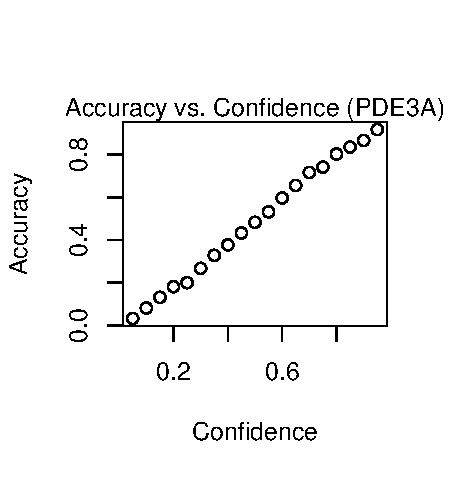
\includegraphics[width=0.3\textwidth]{figures/calibration_plots/pde3a_calib.pdf}
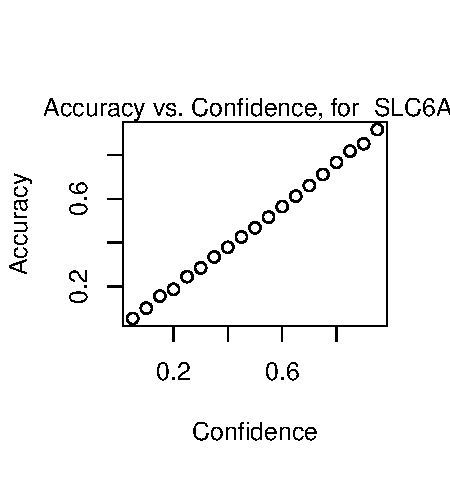
\includegraphics[width=0.3\textwidth]{figures/calibration_plots/slc6a2_calib.pdf}
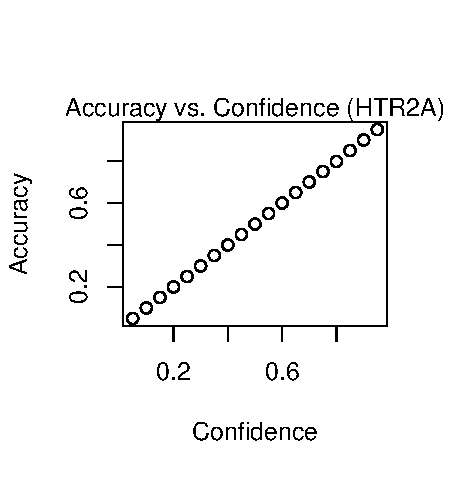
\includegraphics[width=0.3\textwidth]{figures/calibration_plots/htr2a_calib.pdf}
    \caption{Three representative calibration plots, for models PDE3A, SLC6A2
    and HTR2A, based on the smallest, the median, and the largest data sets in
    terms of total number of compounds. The plots show accuracy against
    confidence, for confidence values 0.05 to 0.95 with a step size of 0.05.}
    \label{fig:calibration_plots}
\end{figure}

\subsection{Modeling workflow}
Before the training, the CPSign precompute command was run, in order to
generate a sparse representation of each target's dataset.
ACPs consisting of 10 models were then trained for each target using the CPSign software using the 'train' command.
The cost value used was the one obtained from the hyperparameter tuning. 
% (See \href{https://github.com/pharmbio/ptp-project/blob/c529cf307593c40e7f822a92b224036894c95de1/exp/20180426-wo-drugbank/wo_drugbank_wf.go#L69-L101}{here}).
The computational workflows for orchestrating the extraction of data, model building, 
and the collection of results for summarization and plotting were
implemented in the Go programming language using the SciPipe workflow library 
that is available as open source software at
\href{http://scipipe.org}{scipipe.org} or \href{https://github.com/scipipe/scipipe}{github.com/scipipe/scipipe}.
The cost values for each target is stored in the workflow code, available on github (https://github.com/pharmbio/ptp-project).

\todo{We need an illustration of the workflow, either generated by software or a manually drawn figure}



\subsection{Model validation}

In order to validate the predictive abilities of the trained models, data about
1000 compounds were withheld from the ExcapeDB dataset. The compounds chosen to
be withheld were the following: i) all small molecules in DrugBank (version
5.0.11) with status ``withdrawn'', for which we could find either a pubchem ID
or a CHEMBL ID, ii)  a randomly selected subset of the remaining compounds in
DrugBank 5.0.11, with status ``approved'', for which we could also find PubChem or CHEMBL IDs,
until a total number of 1000 compounds was reached.  No regard was paid to
other drug statuses in DrugBank statuses such as ``investigational''.

\todo{Add info about comparison of results for fillup vs non-fillup? YES! /Ola}

The models built were validated by predicting the binding activity against each
of the 31 targets for all compounds for which we had known binding
data for a particular target. The validation was done with CPSign's validate
command, predicting values at confidence levels 0.8 and 0.9.

\todo{where are these results?}


\section*{Results}

\subsection{Observed fuzziness}

In figure \ref{fig:allmodels_fillup}, performance metrics for each model is
presented in a plot. The plot shows Observed Fuzziness (OF), Class Observed OF
(CNOF) as described in the methods section, training time and validation.

\begin{figure}[h!]
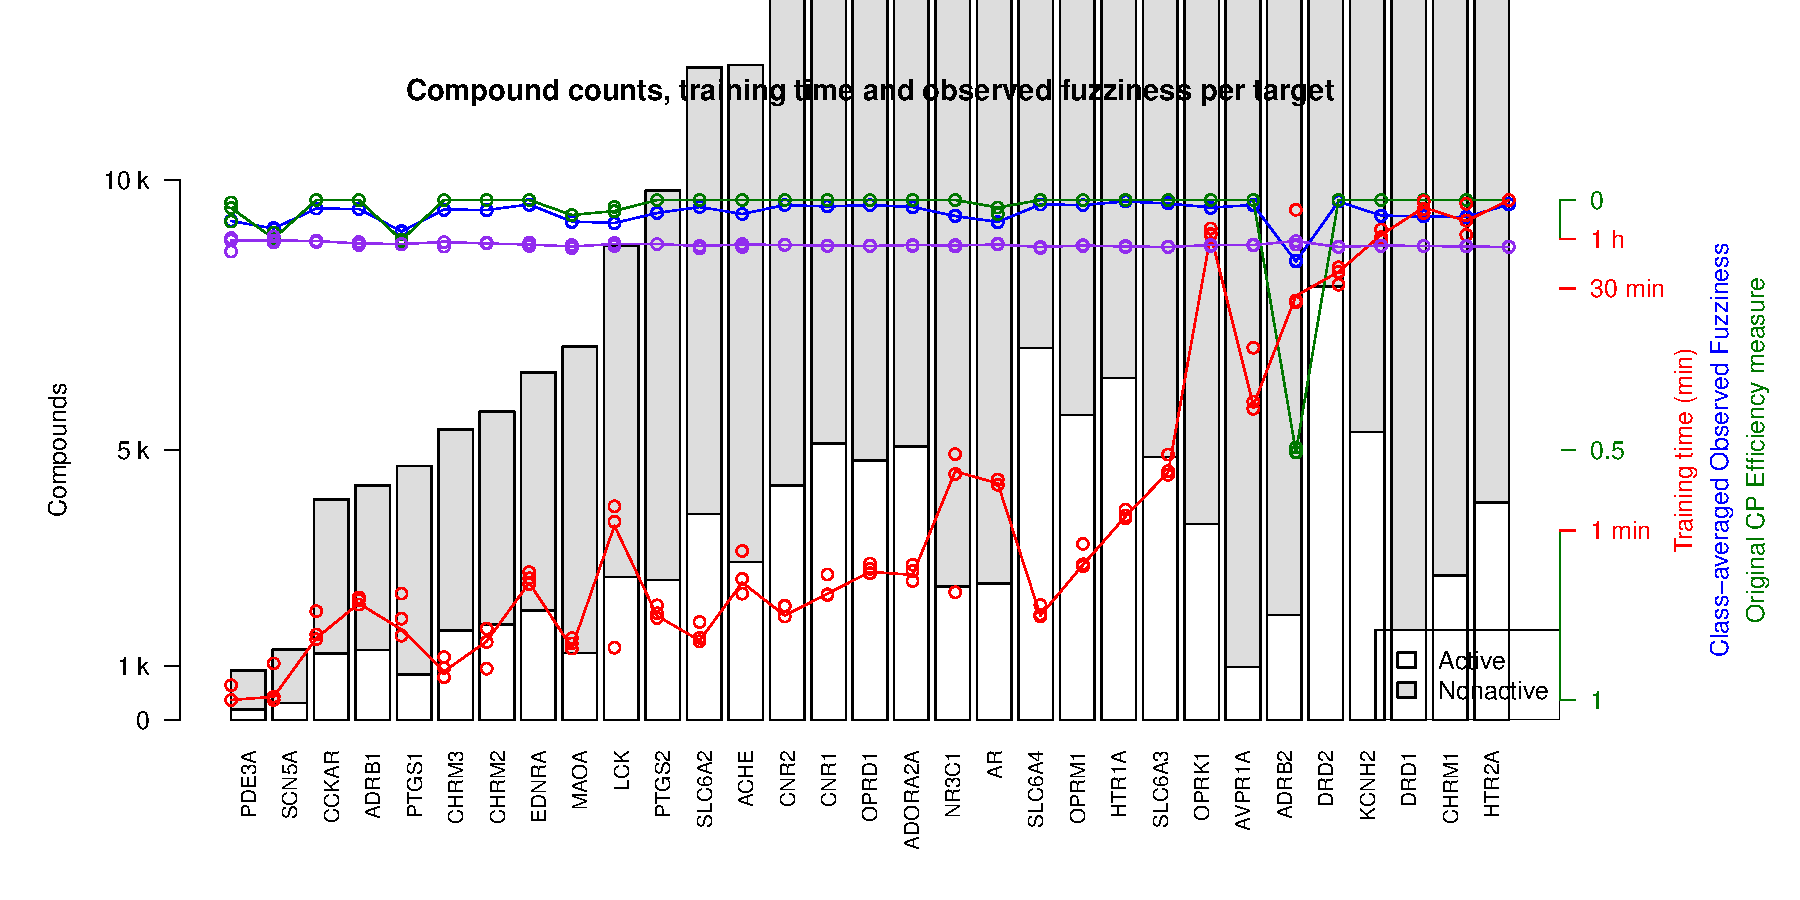
\includegraphics[width=\textwidth]{figures/allmodels_fillup.pdf}
    \caption{All models with the smaller ones being filled up with assumed non-actives. EXTEND FIG CAPTION! }
    \label{fig:allmodels_fillup}
\end{figure}

\begin{figure}
\begin{wideMinipage}
    \begin{minipage}{0.8\textwidth}
    \subbottom[The profile as it looks on the web page. The user draws a molecule, selects a confidence and then the profile updates underneath.]{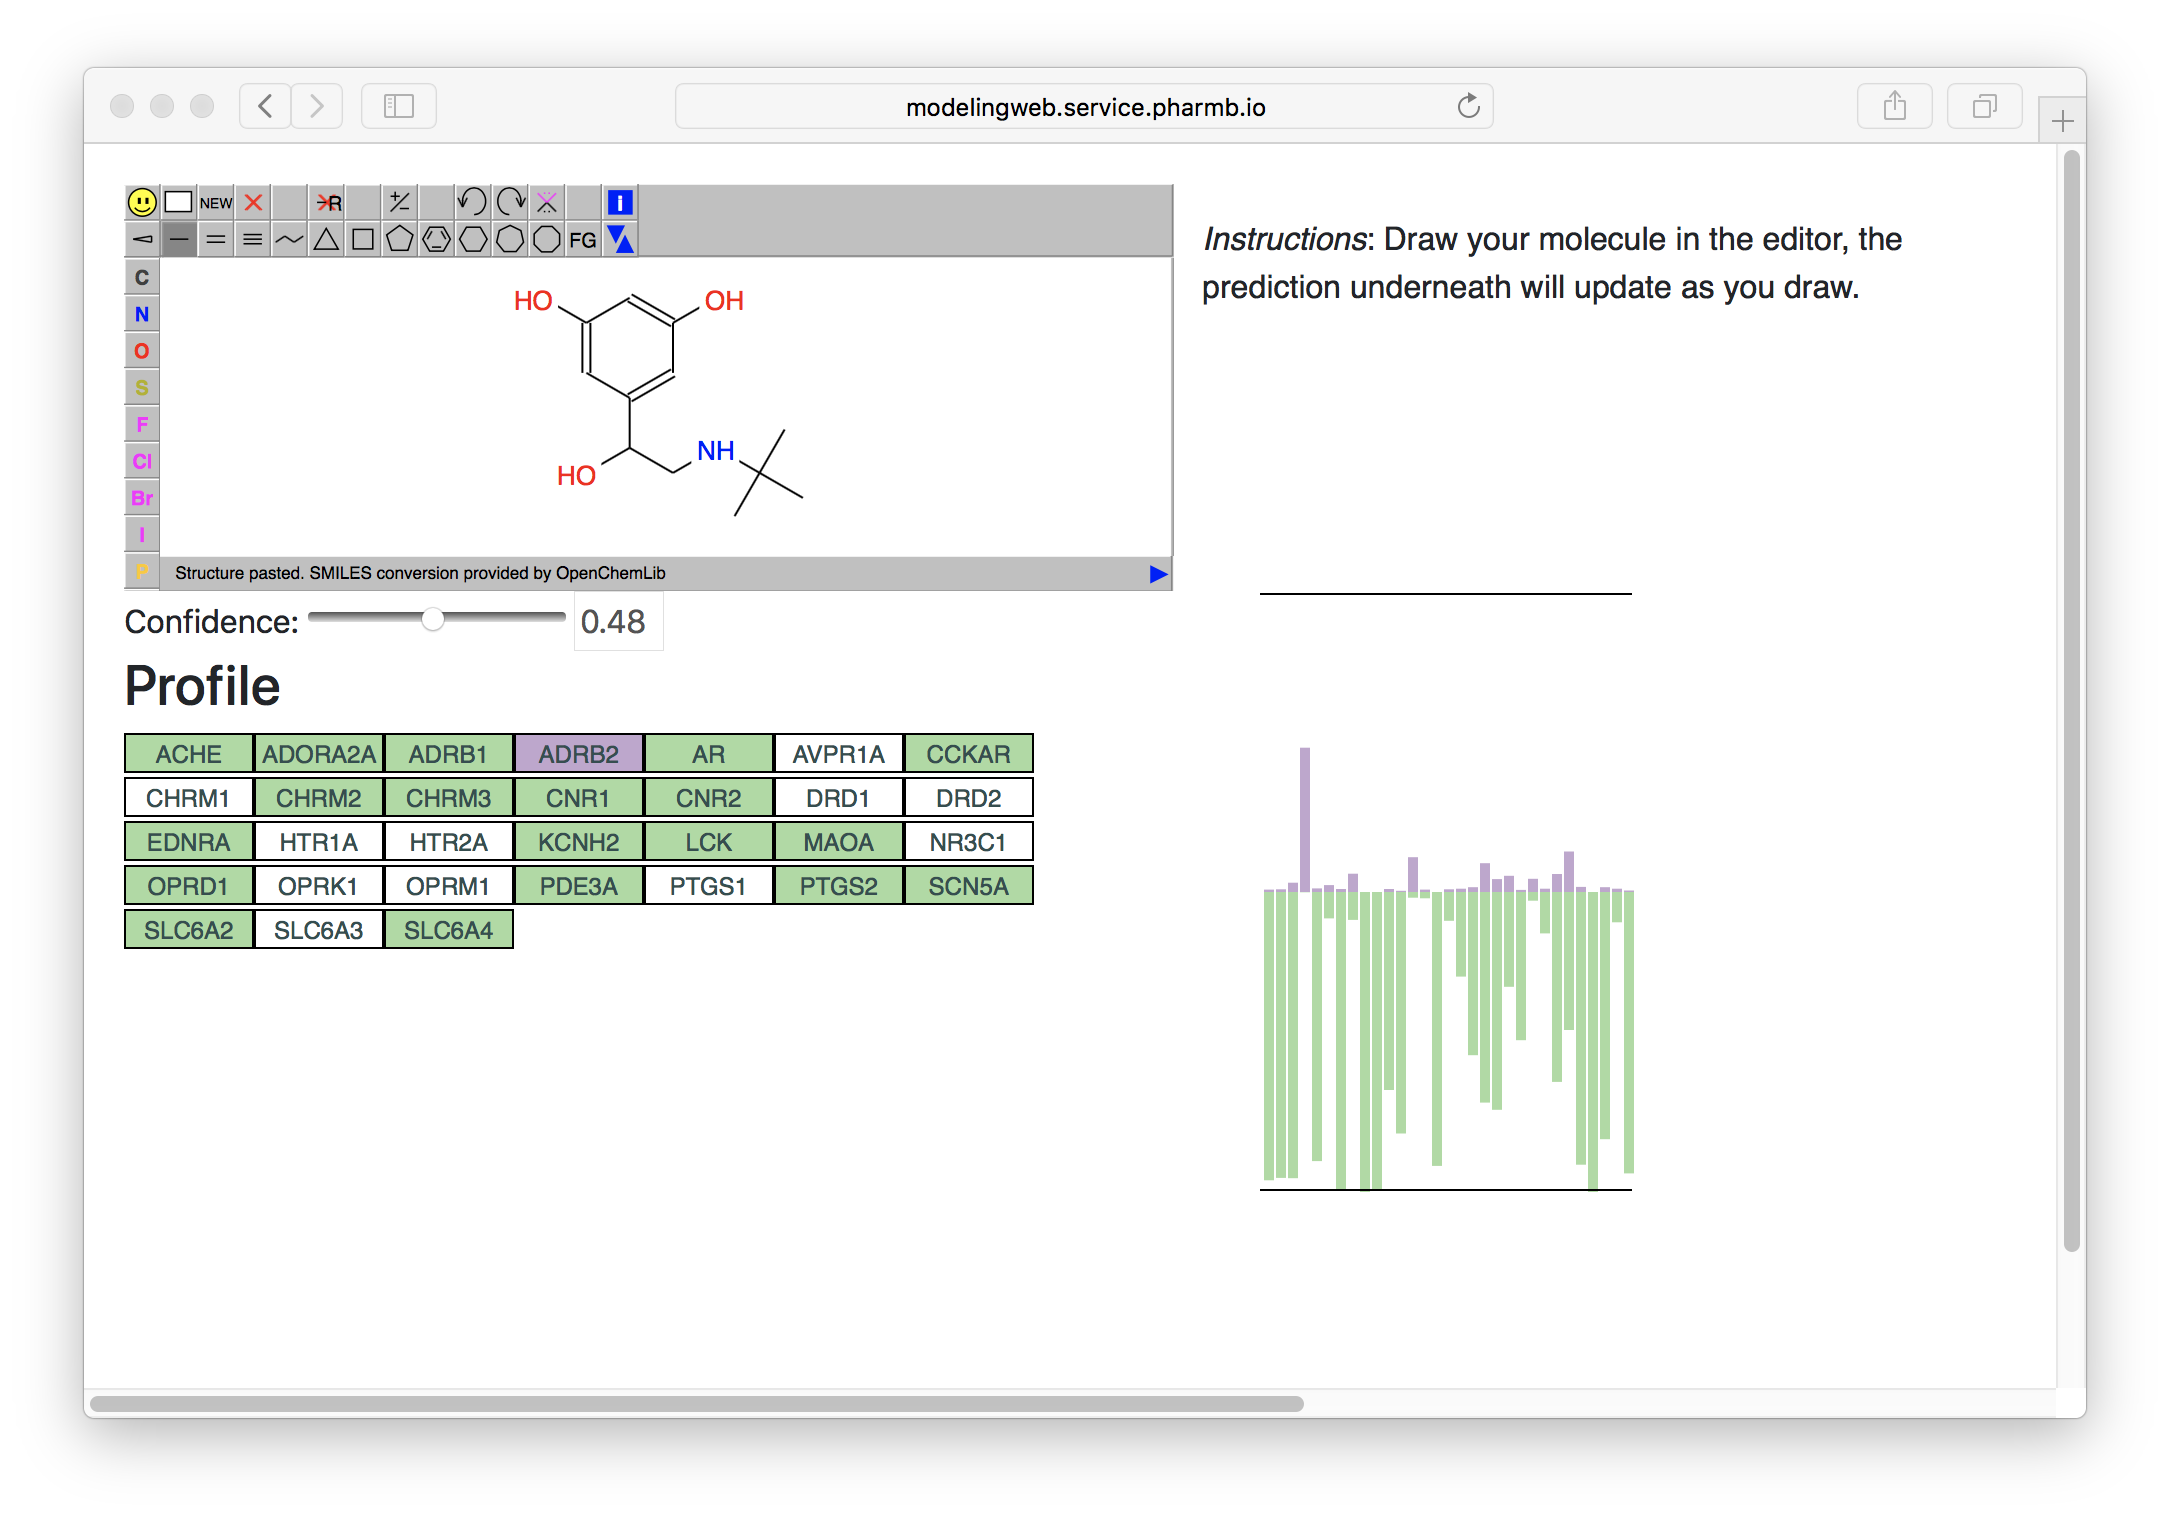
\includegraphics[height=0.41\textheight]{figures/terbutaline.png}}
    \end{minipage}
    \begin{minipage}{0.19\textwidth}
    \subbottom[Coloring of which parts of the molecule contributed the most to the prediction for ADBR2.]{\fbox{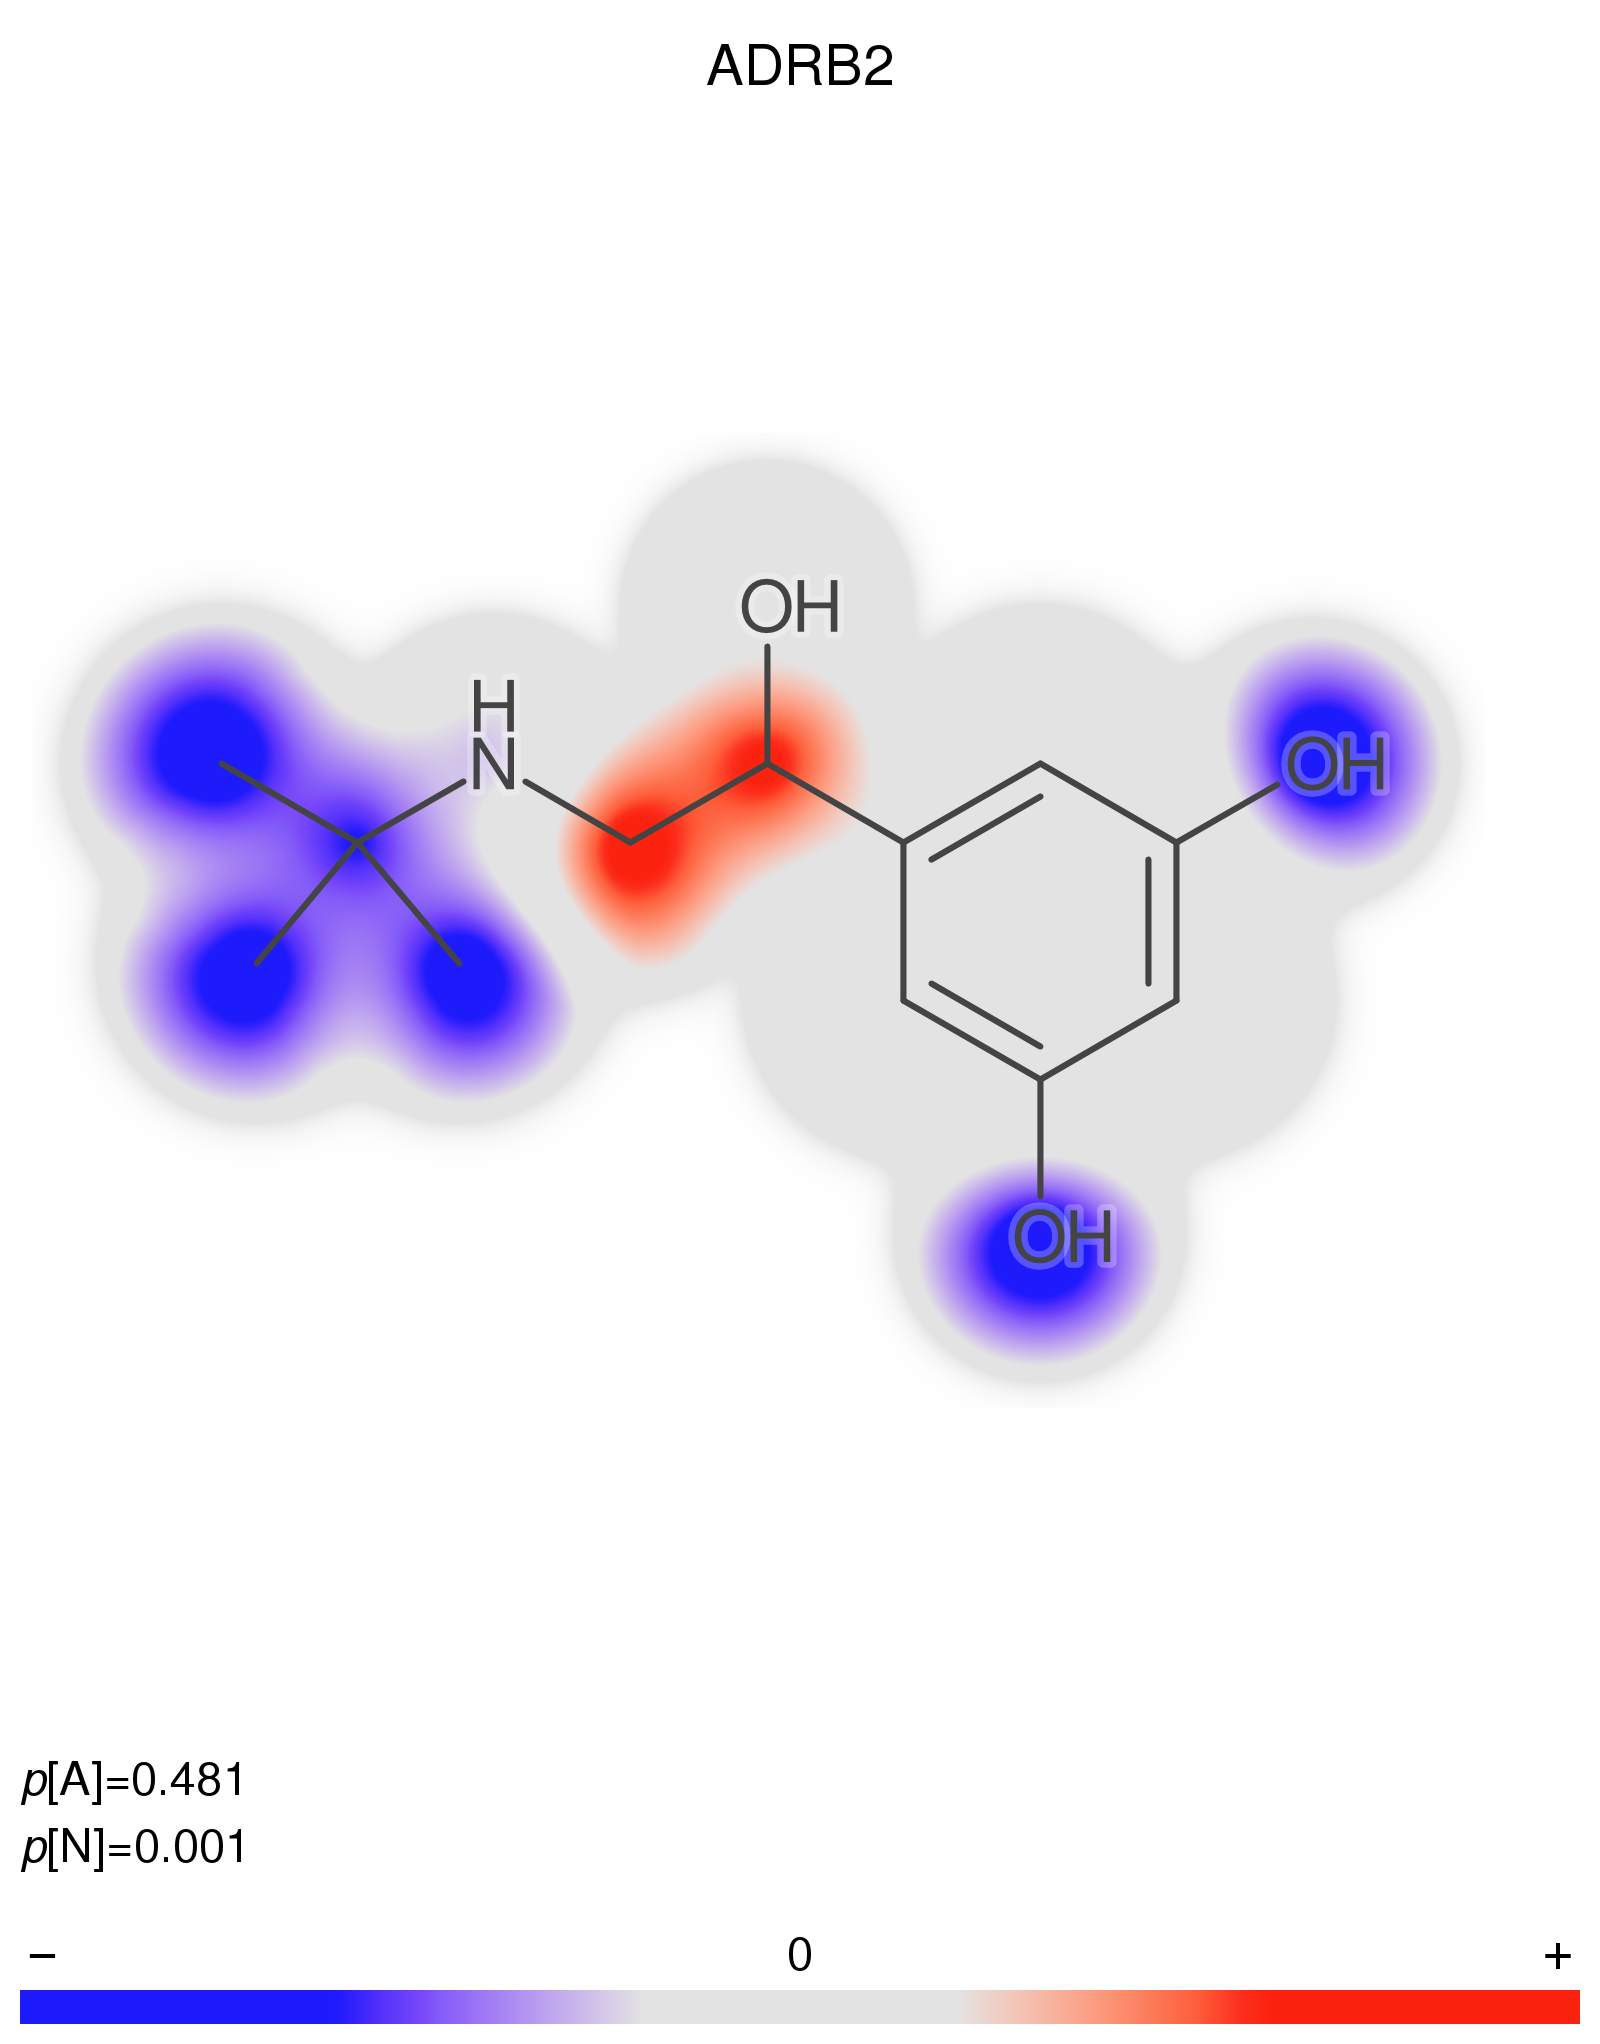
\includegraphics[height=0.22\textheight]{figures/terbutaline2.png}}}
    \end{minipage}
    \caption{The prediction profile for Terbutaline, a known selective beta-2 adrenergic agonist  used as a broncho\-dilator and tocolytic}
\end{wideMinipage}
\end{figure}
\subsection{Changes in class memberships}

\todo{Make a similar plot as Figure 3 in~\cite{Norinder2014}}


\section*{Conflict of Interest Statement}
%All financial, commercial or other relationships that might be perceived by
%the academic community as representing a potential conflict of interest must
%be disclosed. If no such relationship exists, authors will be asked to confirm
%the following statement:
OS, JA, AB, and SA are involved in Genetta Soft AB, a Swedish based company developing the CPSign software.


\section*{Author Contributions}
OS conceived the study. OS, JA, SA and SL designed the study, interpreted results, and wrote the manuscript. SL implemented the workflow and carried out the analysis. SA extended CPSign with new features. JA, SA and AB contributed with model deployment and APIs. EA contributed with expertise in target profiles and cheminformatics. All authors read and approved the manuscript.


%The Author Contributions section is mandatory for all articles, including
%articles by sole authors. If an appropriate statement is not provided on
%submission, a standard one will be inserted during the production process. The
%Author Contributions statement must describe the contributions of individual
%authors referred to by their initials and, in doing so, all authors agree to be
%accountable for the content of the work. Please see
%\href{http://home.frontiersin.org/about/author-guidelines#AuthorandContributors}{here}
%for full authorship criteria.

\section*{Funding}
%Details of all funding sources should be provided, including grant numbers if
%applicable. Please ensure to add all necessary funding information, as after
%publication this is no longer possible.
This study was supported by OpenRiskNet (Grant Agreement 731075), a project funded by the European Commission under the Horizon 2020 Programme.

\section*{Acknowledgments}
%This is a short text to acknowledge the contributions of specific colleagues,
%institutions, or agencies that aided the efforts of the authors.

\bibliographystyle{plain}
\bibliography{ptp}

\section*{Supplemental Data}
%\href{http://home.frontiersin.org/about/author-guidelines#SupplementaryMaterial}{Supplementary
%Material} should be uploaded separately on submission, if there are
%Supplementary Figures, please include the caption in the same file as the
%figure. LaTeX Supplementary Material templates can be found in the Frontiers
%LaTeX folder
%
%

Supplemental 1: Calibration plots for all targets.

\begin{figure}[h!]
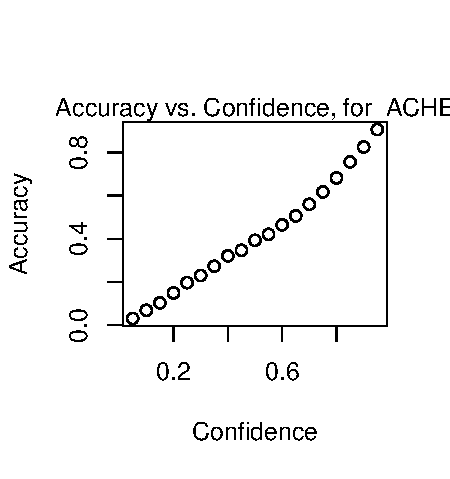
\includegraphics[width=0.19\textwidth]{figures/calibration_plots/ache_calib.pdf}
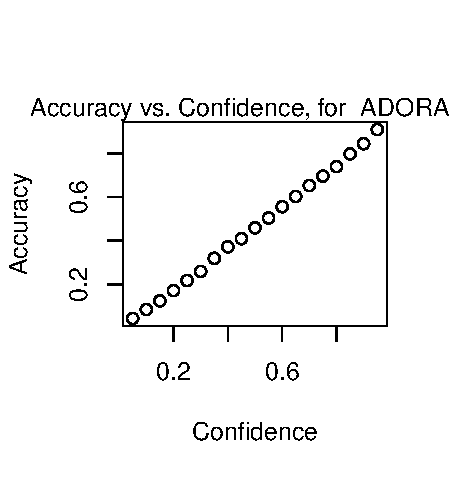
\includegraphics[width=0.19\textwidth]{figures/calibration_plots/adora2a_calib.pdf}
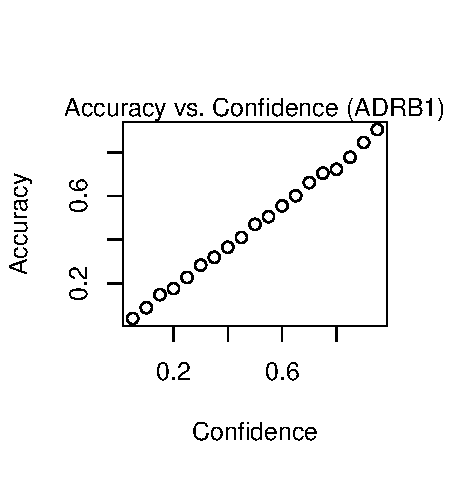
\includegraphics[width=0.19\textwidth]{figures/calibration_plots/adrb1_calib.pdf}
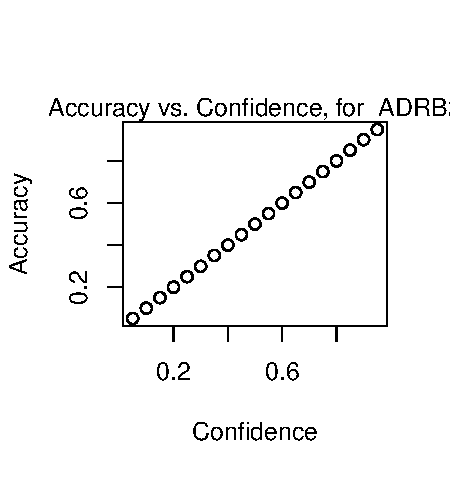
\includegraphics[width=0.19\textwidth]{figures/calibration_plots/adrb2_calib.pdf}
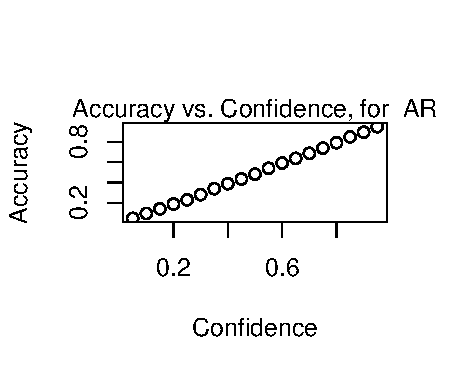
\includegraphics[width=0.19\textwidth]{figures/calibration_plots/ar_calib.pdf}
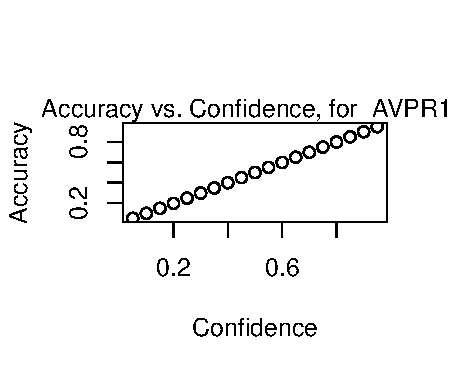
\includegraphics[width=0.19\textwidth]{figures/calibration_plots/avpr1a_calib.pdf}
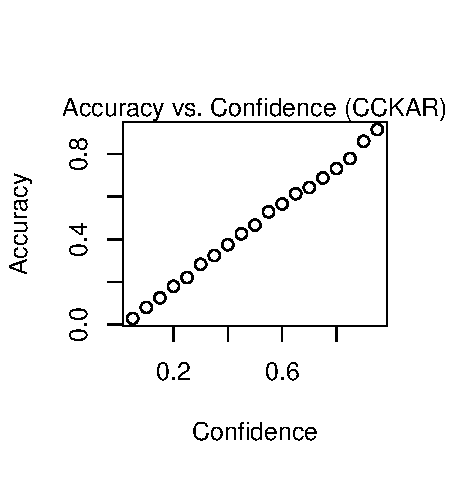
\includegraphics[width=0.19\textwidth]{figures/calibration_plots/cckar_calib.pdf}
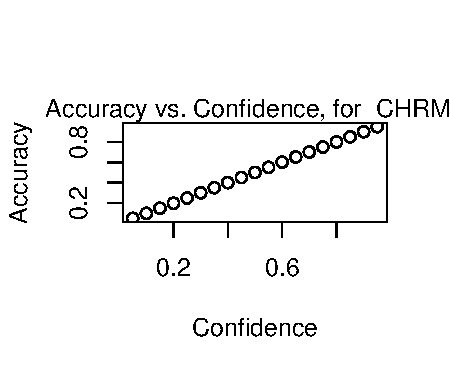
\includegraphics[width=0.19\textwidth]{figures/calibration_plots/chrm1_calib.pdf}
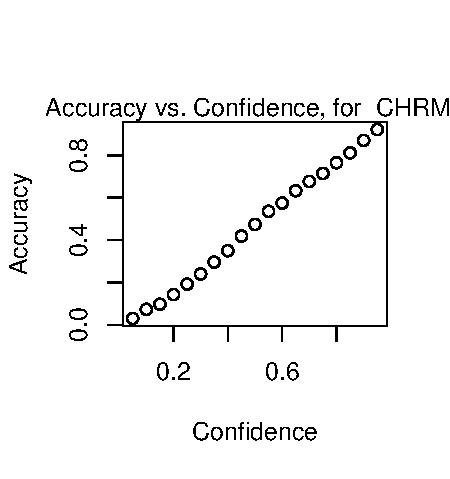
\includegraphics[width=0.19\textwidth]{figures/calibration_plots/chrm2_calib.pdf}
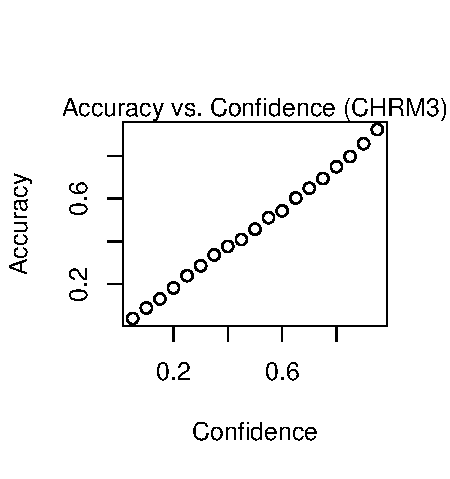
\includegraphics[width=0.19\textwidth]{figures/calibration_plots/chrm3_calib.pdf}
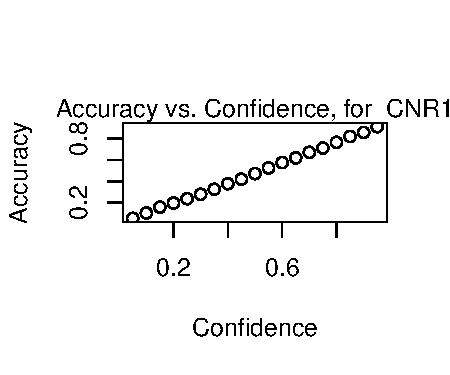
\includegraphics[width=0.19\textwidth]{figures/calibration_plots/cnr1_calib.pdf}
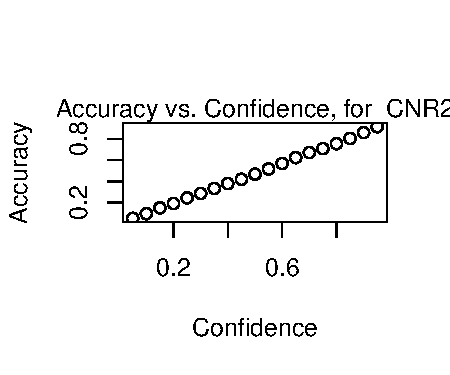
\includegraphics[width=0.19\textwidth]{figures/calibration_plots/cnr2_calib.pdf}
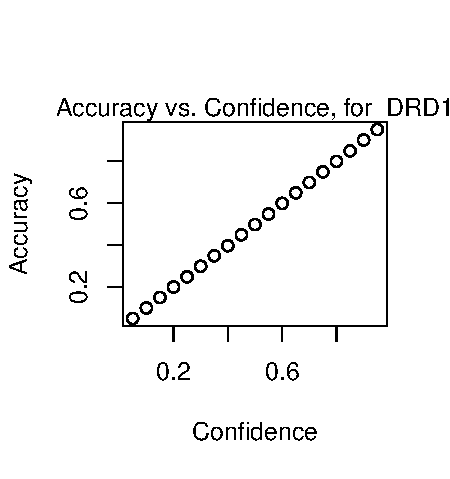
\includegraphics[width=0.19\textwidth]{figures/calibration_plots/drd1_calib.pdf}
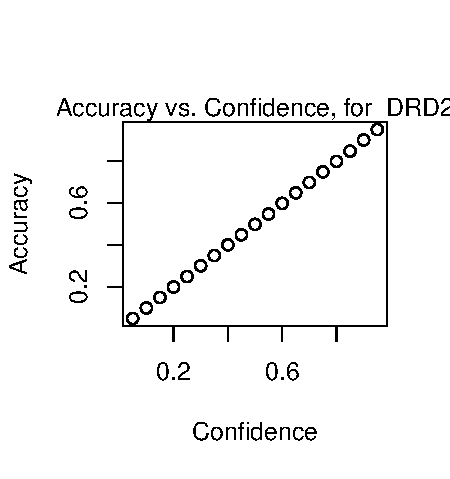
\includegraphics[width=0.19\textwidth]{figures/calibration_plots/drd2_calib.pdf}
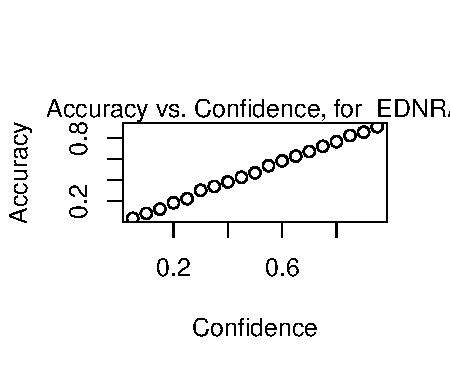
\includegraphics[width=0.19\textwidth]{figures/calibration_plots/ednra_calib.pdf}
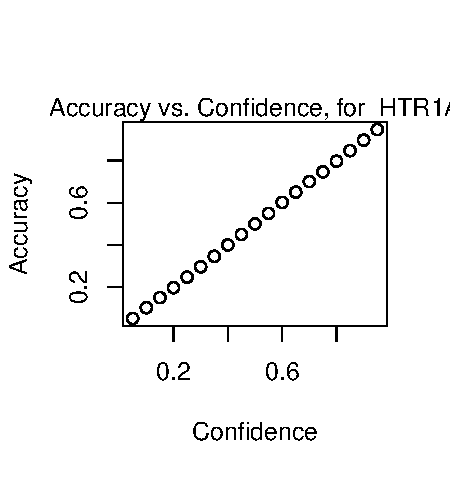
\includegraphics[width=0.19\textwidth]{figures/calibration_plots/htr1a_calib.pdf}
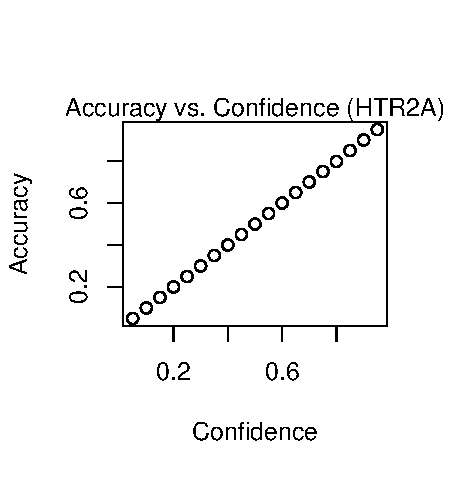
\includegraphics[width=0.19\textwidth]{figures/calibration_plots/htr2a_calib.pdf}
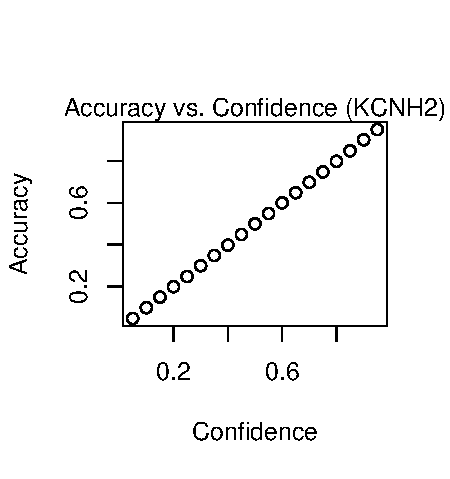
\includegraphics[width=0.19\textwidth]{figures/calibration_plots/kcnh2_calib.pdf}
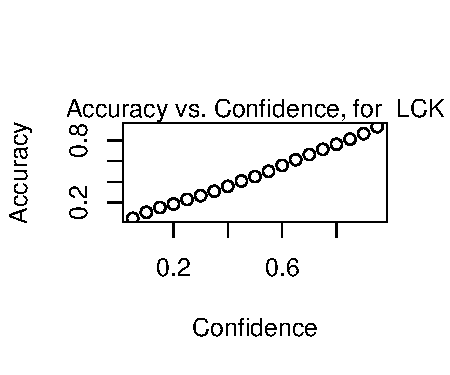
\includegraphics[width=0.19\textwidth]{figures/calibration_plots/lck_calib.pdf}
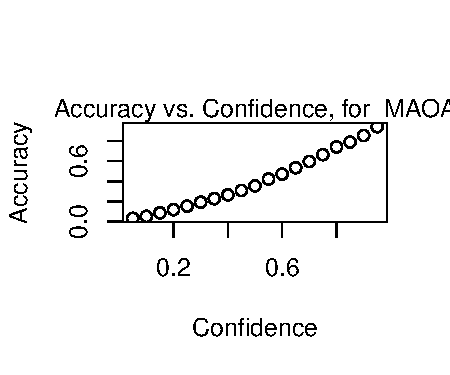
\includegraphics[width=0.19\textwidth]{figures/calibration_plots/maoa_calib.pdf}
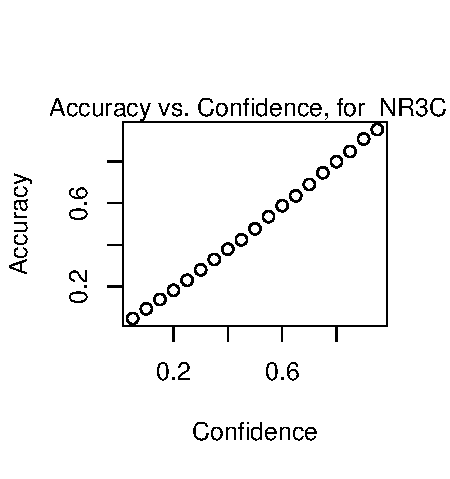
\includegraphics[width=0.19\textwidth]{figures/calibration_plots/nr3c1_calib.pdf}
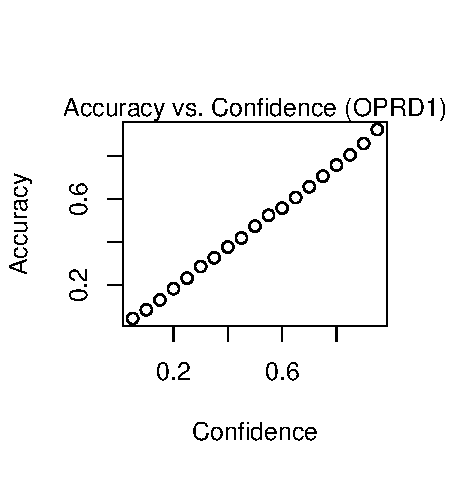
\includegraphics[width=0.19\textwidth]{figures/calibration_plots/oprd1_calib.pdf}
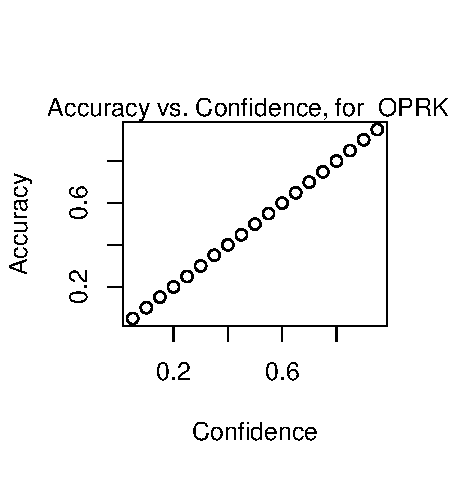
\includegraphics[width=0.19\textwidth]{figures/calibration_plots/oprk1_calib.pdf}
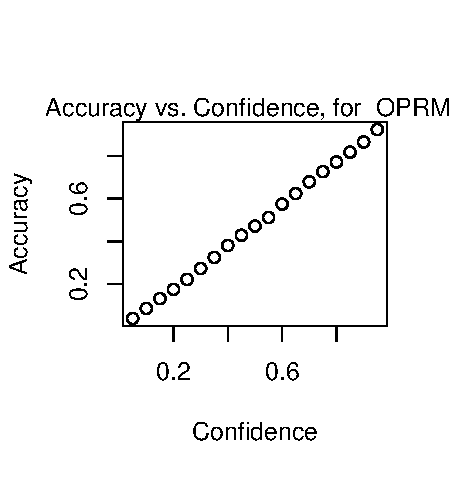
\includegraphics[width=0.19\textwidth]{figures/calibration_plots/oprm1_calib.pdf}
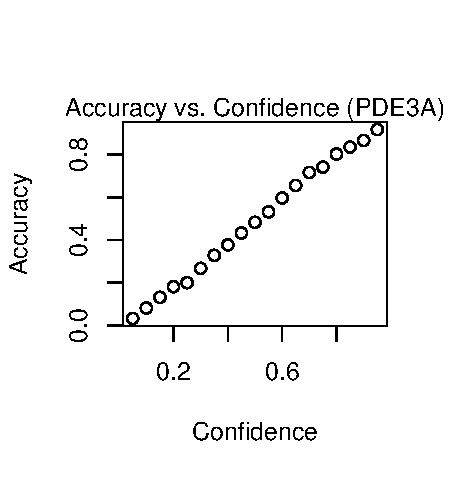
\includegraphics[width=0.19\textwidth]{figures/calibration_plots/pde3a_calib.pdf}
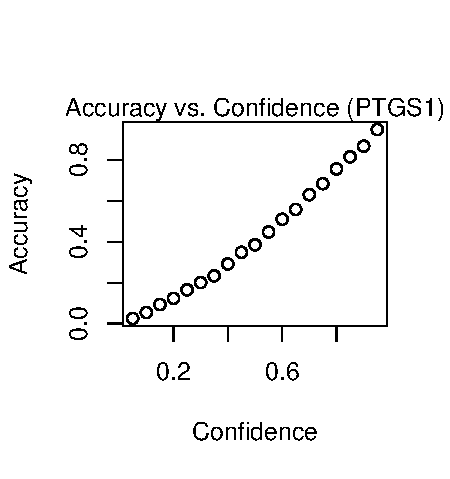
\includegraphics[width=0.19\textwidth]{figures/calibration_plots/ptgs1_calib.pdf}
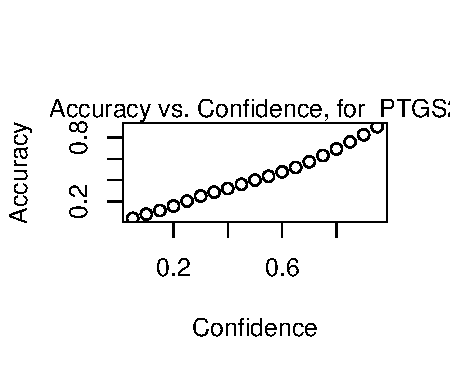
\includegraphics[width=0.19\textwidth]{figures/calibration_plots/ptgs2_calib.pdf}
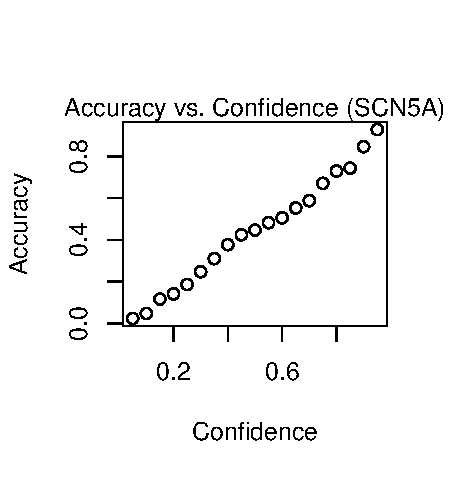
\includegraphics[width=0.19\textwidth]{figures/calibration_plots/scn5a_calib.pdf}
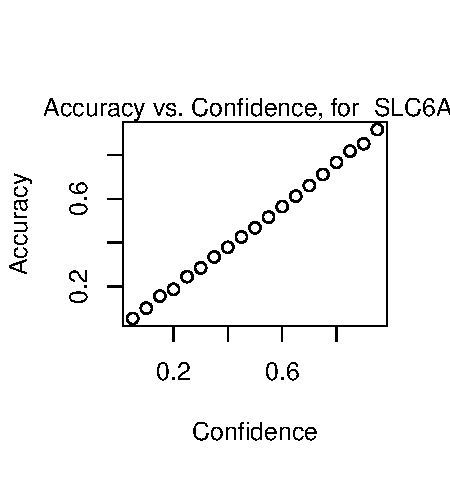
\includegraphics[width=0.19\textwidth]{figures/calibration_plots/slc6a2_calib.pdf}
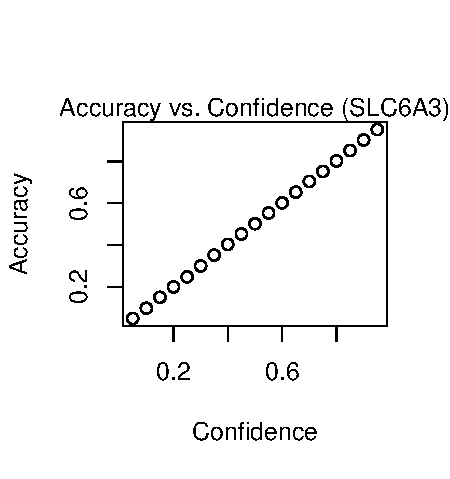
\includegraphics[width=0.19\textwidth]{figures/calibration_plots/slc6a3_calib.pdf}
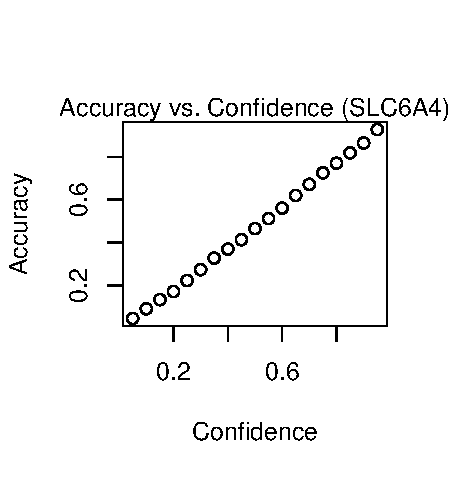
\includegraphics[width=0.19\textwidth]{figures/calibration_plots/slc6a4_calib.pdf}

    \caption{Calibration plots for all targets. The plots show accuracy against
        confidence, for confidence values 0.05 to 0.95 with a step size of 0.05.}
    \label{fig:calibration_plots_all}
\end{figure}
\end{document}
